\subsection{What is projectional editing?}\label{section:WhatIsPE}

Traditionally programmers write code with text editors, or integrated development environments (IDE), which adjust the concrete syntax and allows a parser to create the abstract syntax tree.
A projectional editor, Inverts this relationship, as a developer edits the abstract syntax tree and allows the IDE to project the concrete syntax.

\subsubsection{parser based editing}


In a traditional, parser-based, development workflow, a program is defined using text and can be edited with a text editor.
Because it is text based then the notation of the language is limited to text.
A grammar is a definition of the formal syntactical rules, or concrete syntax, of a programming language.
The lexer and parser are derived from the grammar.
The text is passed into a text buffer where first a lexer will turn the text into tokens. 
A parser will validates that these tokens, the words of the language, are syntactically correct.
If the tokens are not rejected then the parser will construct first a parse, or concrete syntax, tree and from there, an abstract syntax tree (AST).

An AST is a tree structure that represents the semantic meaning of the source code, stripped of all the syntactic details.
The parser will do some name resolution to take care that references within the source code are represented in the tree. 
This turns the tree into a graph.

Compilers use the AST to do subsequent processing, such as linking, transformation, analysis, type checking, etc.
Modern IDEs, in the background, also parse the code it is displaying to create an AST in order to offer relevant coding assistance.
This assistance is appreciated, because without IDE help learning the concrete syntax of large languages is error prone and exploratory programming is laborious if one has to wait until compilation to discover mistakes.


\subsubsection{projectional definition}

In the projectional editing paradigm the program is represented by a semantic model that can only be read and edited with projectional editing tools. 
A projectional editor does not parse any text.
In its place, a developer reads and edits a representation of the AST through a projected notation.
Her editing gestures immediately and directly manipulate the AST within predefined and fixed layouts.

The principle of projectional editing is familiar to those that use visual programming, like Scratch or Blockly, or graphical modelling tools, such as MetaEdit+.
These tools do not parse pixels to get to their AST. 
They project the underlying models/programs in a view and which they store as the model/AST and not as a plain text equivalent in a traditional programming language.

Projectional editing is the generalization of this idea, with the ability to render multiple representation of the program with a wide range of notation styles.

The projection may sometimes seem like a text editor, however this is just acrobatics by the language engineer designing an editor that makes a developer feel more comfortable. 
The text is just another type of projection of the AST.
It also may be any other notation that can represent the semantic meaning of the code, such as formulas, graphs, or images.
Projections are not just the notation, but also how the user interacts with the projection.
In this sense the definition of the projections and the IDE/UI overlap.

\subsection{What is it not[TODO: write this section]}

UML 
MDE
MBSE

Low-code software development

Most confusing of all Projectional Editing the  of projecting an editor from an AST, should not be confused with Projectional Editing the methodology of Product line differentiation in code bases.
The reason we call this confusing is that as well as the name being the same, one of the leading products for this product line technique is called PEoPL, developed in MPS.
This product is a projectional Editor (the paradigm) for product lines projectional editing (the methodology).

\subsubsection{How projectional editing works}

As shown in figure \ref{fig:projectionalEditing_loop}, a projectional editor has a model or an AST. 
It renders a presentation of the model as a projection. 
The developer performs actions on the projection.
every user editing action is directly mapped on to a change in the AST. 

\begin{figure}[h]
    \centering
    \fbox{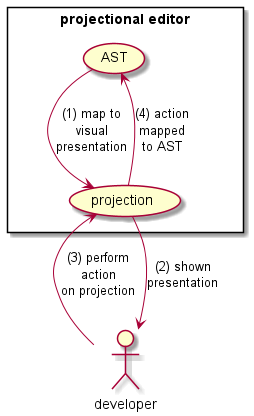
\includegraphics[width=0.35\textwidth]{Sections/images/projections.png}}
    \caption{Projectional editing loop. TODO: comparison with Parsing}
    \label{fig:projectionalEditing_loop}
\end{figure}

To perform the above two things have to be defined by language engineers: The Meta-Model and the editor.

The meta-model, analogous to the abstract syntax, describes the node concepts and connection that can be used to build the, hierarchical structure that is the AST.
This hierarchy can have references to nodes in other branches, so, although named a tree, it is actually a graph.
The AST will be stored independently of the concrete syntax.
The tree is often stored with a database, XML or a proprietary file format.

Rules of the meta-model can further be described through behaviours such as type systems or scoping rules.

Projectional editors avoid the grammars and parsers that serve as the definition of the concrete and abstract syntax in a traditional text based language.
Instead of transforming the concrete to the abstract with parsing, the abstract is transformed to the concrete via a projection engine that uses projection rules.
Editors are a combination of the projection rules and the gestures or actions that will create change request to the AST.
They are analogous to the concrete syntax.

One of the actions can be typing text, however, every string is recognized as it is entered, so there is no tokenizing and the text is being entered into the templates defined in the editor.
The resulting changes are displayed to the developer in a newly derived projection of the underlying AST.

The projection uses graphical elements to represent the representation.
Although often appearing textual, each of the text elements are references to nodes in the AST.

Developers can only interact with the editor via the rigidly controlled code completion menus or gestures and actions. 
    
The AST is directly built from each interaction she has with the editor.
Nodes are creates as instances of the concepts defined in the meta-model.
Each node has it's own unique id and points to it's defining concept.
It is unambiguous.
References are first class and defined by the id rather than resolved by name, as in parser based languages.
Disambiguation happens at time of input, as the developer choses from limited legal inputs.

The separation of the abstract and concrete allows the language engineer to implement multiple projections of the same model, using different notations, each node of the AST taking having the design she envisions.
The pattern used for projection is similar to MVC, so multiple views of the program can be visible and updateable at the same time.

Graphical modelling tools, for example for UML modelling, are specialized implementations of projectional editing.
UML diagrams are not stored as pictures and whose pixels are parsed to create an AST.
Instead the model is stored, often with extra information about visual layout, and the image of the UML is projected to the modeller to edit.
Projectional editing generalizes this approach to projecting any notation defined by the language engineer.



\subsection{Examples of projectional editing}

Table \ref{table:projectional_languages} gives an incomplete and inconsistant history of projectional languages.

\begin{table}[h]
    \begin{center}
        \begin{tabular}{ |l | l | } 
            \hline
            Language                   & Notes   \\
            \hline
            MPS & inspired by a call to action for Language orientated programming\cite{dmitriev2004language} Jetbrains embarked in 2004 \\
                & on a mission to build a product to fulfil that ideal.  Meta Programming System (MPS) was the outcome of that journey.  \\
                & used to create the languages mbeddr, PEoPL, and Realaxy.  Has an active community of deveopers. \\
            Incremental Programming Environment\cite{medina1981incremental}  & A syntax-directed language independent editor from 1980. Got subsumed into GANDALF  \\
            Intentional Domain Workbench & Inspired by Charles Simonyi's 1995 essay ``The Death of Computer Languages, The Birth of Intentional Programming''\cite{simonyi1995death}\\
                    & the IDW was the product of the company Simonyi founded in 2002, Intentional Software. \\
                    & In 2017 Microsoft, as a part of an "acquihire" bought Intentional Software for it's employees and let the product die.\\
            GANDALF\cite{NotkinDavid1985TGp} & Taking over from IPE in 1980 at Carnagie Mellon \\
            Synthesizer Generator & \\
            Whole Platform & \\
            M\'as & \\
            Onion & \\
            Scratch & \\
            Blockly & \\
            Ardublockly & \\
            Kogi & \\
            https://snap.berkeley.edu/ & \\
            Prune & \\
            Eco & \\
            Lamdu & \\
            Blueprints (Unreal Engine) & \\
            Interlisp-D & \\
            deuce & \\
            Enso & \\
            Cedalion & \\  
            Gentleman & \\            
            \hline
        \end{tabular}
    \end{center}
    \caption{An incomplete list of projectional languages}
    \label{table:projectional_languages}
\end{table}


\paragraph{PEoPL}
\paragraph{}
%EXAMPLES
At the same time, projectional language workbenches like MPS [57] and Intentional [47]

Second, Behringer, Palz, and Berger (2017) present Projectional Editing of Product Lines (PEoPL), a DSL that enables multiple projections for variability mechanisms.

Such editors have existed since the 1980s and gained widespread attention with the Intentional Programming paradigm, which used projectional editing at its core.

Projectional editing, also known as structured editing or syntax-directed editing, is not a new idea; early references go back to the 1980s and include the Incremental Programming Environment [32], GANDALF [35], and the Synthesizer Generator [39].
Work on projectional editors continues today: Intentional Programming [44, 18, 45, 14] is its most well-known incarnation.
Other contemporary tools [20] are the Whole Platform [9], M´as [3], Onion, and MPS [4]

Projectional Editors from the 1980s.
GANDALF [35] and the Incremental Programming Environment (IPE) [32] do not attempt to make editing textual notations efficient; for example, they lack support for linear editing of tree-structured expressions.
The Synthesizer Generator [39] avoids the use of projectional editing at the fine-grained expression level, where textual input and parsing is used.
While this may improve editing efficiency, it risks the advantages of projectional editing, because language composition at the expression level is limited.
Another work that implements and uses a DSL within the Synthesizer Generator [37] concludes: “Program editing will be considerably slower than normal keyboard entry, although actual time spent programming non-trivial programs should be reduced due to reduced error rates.”

The Intentional Domain Workbench (IDW) is the most recent implementation of the Intentional Programming paradigm [44, 18], supporting diverse notations [45, 14].
Since it is a commercial, closed-source project without widespread adoption yet, we cannot easily study it or survey its users.


All contemporary projectional editors are part of language workbenches

An early example of a projectional editor is the Incremental Programming Environment (IPE) [16].
It supports the definition of several notations for a language as well as partial projections, where parts of the AST are not shown.
However, IPE did not address editor usability; to enter 2+3, users first have to enter the + and then fill in the two arguments.
Another early example is GANDALF [17]; the report in [20] states that the authors experienced similar usability problems as IPE: “Program editing will be considerably slower than normal keyboard entry, although actual time spent programming non-trivial programs should be reduced due to reduced error rates.”
The Intentional Programming project [9, 22] has gained widespread visibility and has popularized projectional editing; the Intentional Domain Workbench (IDW) is the contemporary implementation of the approach.
IDW supports diverse notations [7, 23].

Scratch [15] is an environment for learning programming.
It uses a projectional editor, but does not focus on textual editing; it relies mostly on nested blocks/boxes.
So does GP [18].
Textual notations, and thus grammar cells, are not relevant.
Prune [2] is a projectional editor developed at Facebook.
The goal is explicitly to not feel like a text editor; the hypothesis is that tree-oriented editing operations are more efficient than those known from text editors.
While this is an interesting hypothesis, our considerable experience with using projectional editing in real projects has convinced us that this approach is not feasible; hence the work described in this paper.

The Synthesizer Generator [21] is a projectional editor which, at the fine-grained expression level, uses textual input and (regular, textual) parsing.
While this improves usability, it destroys many of the advantages of projectional editing in the first place, because language composition and the use of non-textual notations at the expression level is limited.

Eco [10] relies on language boxes, explicitly delineated boundaries between different languages used in a single program (e.g., the user could define a box with Ctrl-Space).
Each language box may use parsing or projection.
This way, textual notations can be edited naturally, solving the usability issues associated with editing text in a projectional editor.

*** gothere
Lamdu [5], a functional, projectional language (no paper)

. Dataflow visual programming languages, such as Blueprints in the Unreal Engine [2], are often domain-specific.


Early syntax-directed source code editors included Interlisp-D (for Lisp’s limited syntax) and Emily[1] (for PL/I’s rich syntax).

deuce: lightweight structured editing in sketch-n-sketch

Blockly: https://developers.google.com/blockly

mage? r Jupyter notebooks

citrus
visual macro system in Racket


An early example of a ProjE is the Incremental Programming Environment (IPE) [4].
Another early example is GANDALF [5], which generates a ProjE from a language specification.

The Synthesizer Generator [7] is also a ProjE.
However, at the fine-grained expression level, textual input and parsing is used.
While this improves usability, it destroys many of the advantages of projectional editing in the first place, because language composition at the expression level is limited.
In fact, extension of expressions is particularly important to tightly integrate an embedded language with its host language [8].

The Intentional Programming [2,3] project has gained widespread visibility and has popularized projectional editing; the Intentional Domain Workbench (IDW) is the contemporary implementation of the approach.
IDW supports diverse notations [9,10].


Language boxes [11] rely on explicitly delineating the boundaries between different languages used in a single program (e.g., the user could change the box with Ctrl-Space).
Each language box may use parsing or projection.


according to LWBC 2015 the 4 porjectional LWB that took place Enso, Mas, MPS, and whole


Cedalion's 







\subsubsection{What advantages does projectional editing bring?}

Projectional editing gives advantages both to the language engineer and the program developers.
There is a lot of crossover and repetition between papers written on the subject of projectional editing as to the advantages it brings.
To that end, what follows is a synthesis of a number of papers as to the advantages given.
Rather than attributing advantages in line to their citations, a helpful reference of papers which proclaim such advantages can be found in table \ref{table:Projectional_Advantages}.

\begin{table}[h]
    \begin{center}
        \begin{tabular}{ |l | c | l | } 
            \hline
            Advantage                   & \#& Paper(s)   \\
            \hline
            Exploratory programming     & 5 & \cite{klimevs2016domain,ratiu2017experiences,volter2010language,voelter2014towards,hosseinkord2021code}                                                                        \\
            Correctness-by-construction & 7 & \cite{voelter2013dsl,ratiu2019fasten,ratiu2012language,klimevs2016domain,berger2016efficiency,klimevs2016domain,vysoky2018ingrid}                                          \\
            Rich notation               & 22& \cite{pech2021jetbrains,voelter2014supporting,voelter2010language2,voelter2015using,voelter2010embedded,guttormsen2017consistent,voelter2010domain,wortmann2016domain,klimevs2016domain,voelter2013mbeddr,berger2016efficiency,simonyi2006intentional,voelter2016efficient,vysoky2018ingrid,pech2013jetbrains,volter2010language,voelter2014projecting,ratiu2018taming,voelter2015towards,voelter2014towards,simonyi1995death,voelter2019using} \\
            Mixed notation              & 8 & \cite{ratiu2017experiences,voelter2010language2,voelter2015using,voelter2010embedded,guttormsen2017consistent,volter2010language,voelter2014supporting,voelter2014towards}              \\
            Multiple views              & 9 & \cite{klimevs2016domain,voelter2016efficient,voelter2010language2,volter2010language,voelter2010embedded,voelter2010domain,vysoky2018ingrid,volter2010language,voelter2014supporting}   \\
            Language composition        & 23& \cite{voelter2013dsl, meacham2020adaptivevle, ratiu2019fasten, pavletic2013extensible,voelter2011language,guttormsen2017consistent,berger2016efficiency,voelter2016efficient,voelter2010embedded,ratiu2012implementing,volter2010language,voelter2010language2,voelter2012mbeddr,voelter2011product,voelter2013requirements,voelter2014supporting,voelter2014towards,voelter2015using,voelter2019using,simonyi1995death,vysoky2018ingrid,pech2013jetbrains,voelter2015towards} \\
            IDE functionality           & 4 & \cite{klimevs2016domain,voelter2010embedded,voelter2010language2,voelter2010embedded}                                                                                                \\
            Language evolution          & 1 & \cite{schindler2016language} \\
            Ancillary data              & 5 & \cite{voelter2011product,voelter2013requirements,voelter2019using,volter2010language,voelter2010language2} \\
            \hline
        \end{tabular}
    \end{center}
    \caption{Papers describing advantages.}
    \label{table:Projectional_Advantages}
\end{table}

 
\paragraph{Exploratory programming}
As with their progenitors, syntax-directed editors, modern projectional editors help guide a developer unfamiliar with a language.
The defined editors with rigid syntax and pre-defined layout mean that only specific cells within the editor can be edited.
This template style means the she does not have to worry about significance of spacing or indentation.
Minutiae of syntactic adornments, such as statement ending semi-colons or enclosing matched brackets, are also not interfering with her exploration of the language space.

When creating code the developer is only presented with legal options within the current context.
As the projection is context aware, relevant actions or options can be suggested and irrelevant ones can be removed.
Thus, it is easier for her to explore which options and actions the language allows her to choose.
Intelligent code completion does not have to be limited to single nodes. 
Whole subtrees can be inserted allowing the developer to explore the larger structures of the language.

\paragraph{Correctness-by-construction}
A projectional editor, by controlling the interaction between the developer and the AST, prevents her from writing syntactically incorrect code.
The whole class of syntactical errors are made impossible, with the developer relieved of having to think about special characters and layout.
Typing and scoping errors are removed by only allowing validly typed and scoped options for the developer.

The developer is only able to select statements that are legal in the context of the location within the AST.
Code does not have to be disambiguated, as this happens at time of entry by the developer.
If there are multiple items that share the same presentation in the editor, the developer chooses the relevant item, resolving the ambiguity to what she means rather than what the parser thinks she means.

\paragraph{Rich notation}
The choice of projection is unconstrained by the restrictions of code that needs to be parsed from a textual source.
This freedom opens up diverse otherwise difficult or impossible to parse notations.
Examples include tabular, mathematical expressions and symbols, diagrams, trees, images, forms, prose, sub- and superscript.
Any visual form or shape that can be mapped to the AST can be used to represent the program in an editor.

With these notations one can better reflect the semantics of the program domain, which should aid comprehension.
Mathematics has a rich history of use of notation.
When writing a DSL for the Mathematics domain, the domain experts can interact with it in the centuries old language of their domain. 

Of course the projections can also be projections of text.  
This is often the appropriate projection type if the developer interacting with the language's domain expertise is parser-based languages.

\paragraph{Mixed notation}
Because no parsing is required, the different forms of rich notation can be combined without the need to create a unifying parser.
With all notations working on the same editor infrastructure mathematic symbols can be embedded within textual projections, within tables within graphical representations.
As ambiguity is not an issue for the underlying AST, then mixing different notations becomes much easier.

\paragraph{Multiple views}
With the AST being the stored artefact rather than the notation, projectional editing allows the language engineer to define multiple views on the same model optimised for different tasks.
Similar to how software architecture presents different views for different stakeholders interests, the same notational diversity can be achieve with specific editors targeted to experts in the various parts of the domain.
A developer can switch between different projections of a node within a larger projection, to find the one that best suits their current task.

Because the architecture of a projectional editor follows the principles of model view controller, it is possible to have multiple simultaneous views of the model.
This allows the developer to update a projection that is optimised for writing and immediately see its effect in a projection optimised for understanding.

\paragraph{Language composition}
Parser-based languages can support some modularization and composition, but a projectional editor allows easy and extensive modular language extension and composition.
This is a result of the nodes of an AST being disambiguated at entry rather than through a parser.
If two items with the same syntax are available at the same place, then the user will choose the one that they require, and therefore the node has an explicitly chosen meaning.

The composition of independently developed languages does not suffer from the syntactic or keyword clashes they would in two grammar defined languages.
Because of the lack of ambiguity, every node referencing the concept that defines it, these languages, when put together, will not have structural or syntactic issues.

Composition can involve extending an existing language or embedding other languages in a host language without modifying the definition of said language.
The ease of composition and extensions leads to the advantage of being able to build larger languages out of smaller modules.

\paragraph{IDE functionality}
Developers in mature languages are used to the functionality of mature IDEs.
These functionalities include syntax highlighting, intelligent code completion or suggestion, and static analysis for errors and validation.
As projectional languages store the AST rather than the the concrete syntax, they require an IDE to edit.
Because of this, when a language engineer designs the language she also has to design the IDE.

Because the projection is based on the AST it always knows it's context.
When the editor already knows the meaning of the node it is representing, then syntax highlighting is simple.
From knowing it's context, it makes it much simpler to suggest intelligent code completions.

Always having a complete AST makes it much easier to validate scope, typing and other hard to implement code validators.

\paragraph{Language evolution}
Parsing complicates the evolution of languages, for example, adding a new reserved word is difficult without breaking existing code.
Extending a language with new capabilities and syntax in projectional editing is simple.
If the change is syntactic then the language engineer has to update an editor.
If there is a semantic change then the language engineer can write a migration in the language, to transform a node of one concept to a different type, and the developer would have to run that migration on their code.

\paragraph{Ancillary data}
Data can be added to nodes that can augment the AST. 
This has shown to be useful for documentation, requirements traceability and product line feature dependencies.

\subsubsection{What are the disadvantages of projectional editing?}
Whilst there are fewer papers proclaiming the disadvantages of projectional editing, we repeated the approach of the previous section.
Thus, we have synthesised the disadvantages from papers in the following sections and listed citations for these ideas in the table \ref{table:Projectional_Disadvantages}

We do not consider that the dearth of disadvantages discussed as evidence of projectional editings superiority.
We consider that those who do not find projectional editing useful do not write papers about it.

\begin{table}[h]
    \begin{center}
        \begin{tabular}{ |l | c | l | } 
            \hline
            Disadvantage               & \#& Paper(s)   \\
            \hline
            Low adoption               & 4 & \cite{vysoky2018ingrid,voelter2015using,voelter2015towards,voelter2014projecting} \\
            Unnatural user experience  & 11 & \cite{vysoky2018ingrid,voelter2015towards,voelter2014towards,voelter2012mbeddr,voelter2014projecting,berger2016efficiency,voelter2016efficient,voelter2010embedded,voelter2010language2,schindler2016language,voelter2014supporting} \\
            Abigious syntax           & 1 & \cite{guttormsen2017consistent} \\
            Inflexibility              & 2 & \cite{voelter2014towards,voelter2014supporting} \\
            lack of integration with text ecosystem & 5 & \cite{voelter2012mbeddr,voelter2014towards,voelter2012mbeddr,voelter2014projecting,voelter2014supporting} \\
            Learning curve             & 5 & \cite{voelter2010language2,pech2013jetbrains,voelter2012mbeddr,voelter2014towards,voelter2015using,prinz2021teaching} \\
            Vendor lock\-in            & 2 & \cite{voelter2010embedded,voelter2010language2,tomassetti2020reflections} \\
            \hline
        \end{tabular}
    \end{center}
    \caption{Papers describing projectional editing disadvantages.}
    \label{table:Projectional_Disadvantages}
\end{table}

\paragraph{Lack of adoption}
The ideas that proceeded projectional editing - structured editor or syntax-directed editor - has been around since the early 1970's yet has failed to be adopted widely.
This argument is a bit of a tautological one, as the low adoption is perhaps an outcome of the other disadvantages of projectional editing.
However, low adoption can lead to a viscious circlem where lack of adoption prevents further adoption.

\paragraph{Inconvenient or unnatural editing}
Early attempts at projectional editing presented an inconvenient and unnatural user experience when coding.
These usability challanges, exempified by the tedious manner of entering code as per the order of the tree, compares badly to parser based languages.
A traditional text based language can be entered the way it looks, by typing the characters one after another,

This bad reputation continues, despite massive improvements in projectional editors.
Whilst there is no debate that projectional editing feels different, it is questioned as to whether this inconvenience is an intrinsic property or a result of developers, through year of experience, being used to text based programming. 

Modern projectional editors, when using a textual syntax face an "uncanny valley" issue.
Whilst trying to simulate a text editor, the developers start to expect all of the functinoality of the text based IDEs.
This is a particular weak spot, especially with regards to granularity and restrictions of cursor movement, insertion, deletion, selection, copy and pasting, and other interacting with text

\paragraph{Ambigious syntax}
One of the selling points of projectional editing, especially when it comes to language composition, is that there can be no ambigious syntax.
Whilst this may be true for the AST, it is not so for the developer as they read this code on the screen.
If one combined Drools and Basic rather than Java, the developer may become confused as to which language the ``Then'' keyword referes when she read it.

\paragraph{Inflexibility}
As a developer one has no flexibility in code layout, perhaps for enhanced readability. 
This is entirely in the hands of the language engineer when determining the projection rules.

\paragraph{Integration with the text based world}
Projectional editors do not store the definition of the program in the form of a plain text implementation in the concrete syntax.
Instead the AST is stored and serialized in a format not meant to be human readable, such as XML.

This leads to an issue with integration with the infrastructure that has grown arounf text based programing languages.
Two notable examples are text diffing, especially where branch merging is concerned and code sharing.
The diffing issue can and has been solved within projectional editing tools.
This is however difficult to integrate into the workflows of software development workflows that include multiple tools.

Textual source code can be be shared simply by email or websites, this is not the case with projectional code.

\paragraph{Learning curve}
For the language engineer, the necessity to develop an editor with a good user experience is much harder work than defining a grammar for a parsed language.
The learning curve for the langauge engineer is significant, as by default, she has to think also of the IDE devleopment.

For the developer, the different style of editing takes some getting used to.

\paragraph{Vendor lock-in}
The nature of projectional editing is that what one edits is a projection of the AST and therefore an IDE is needed to do the projecting, as well as language definition.
Organisations thinking of going the projectional route for their DSLs may fear being locked into a specific implementation of the concept.
To be able to use previously developed languages would require using the same tool set. 
Changing to a different toolset for language design would require a significant re-skilling effort.





% WIP End